\begin{figure}[htbp]
  \centering
  \resizebox{0.92\textwidth}{!}{%
  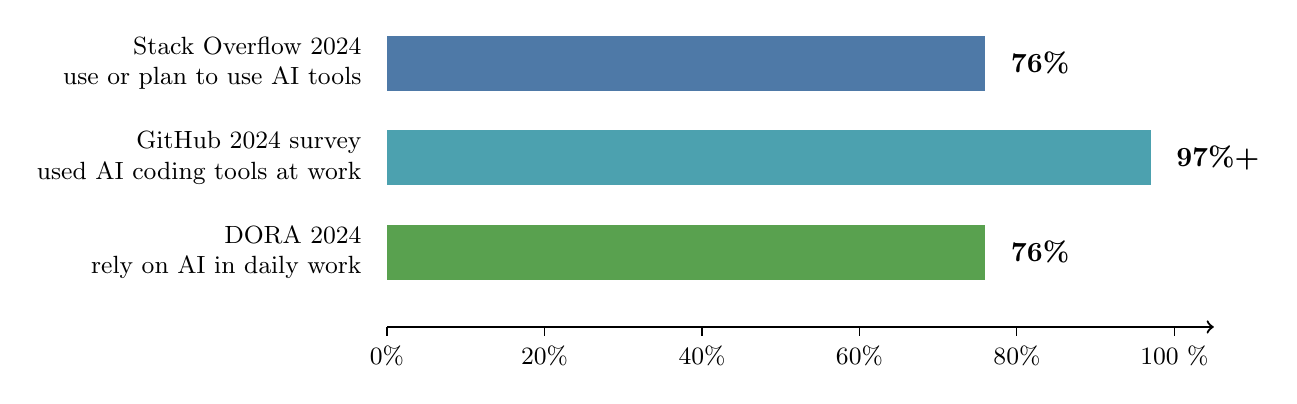
\begin{tikzpicture}[font=\small]
    \definecolor{adoptblue}{RGB}{78,121,167}
    \definecolor{adoptteal}{RGB}{76,161,175}
    \definecolor{adoptgreen}{RGB}{89,161,79}

    \draw[->, thick] (0,0) -- (10.5,0);

    \foreach \x/\label in {
      0/0,
      2/20,
      4/40,
      6/60,
      8/80,
      10/100
    }{
      \draw (\x,0) -- (\x,-0.12);
      \node[below] at (\x,-0.12) {\label\%};
    }

    \fill[adoptblue] (0,3.0) rectangle (7.6,3.7);
    \fill[adoptteal] (0,1.8) rectangle (9.7,2.5);
    \fill[adoptgreen] (0,0.6) rectangle (7.6,1.3);

    \node[anchor=east, align=right] at (-0.2,3.35) {Stack Overflow 2024\\use or plan to use AI tools};
    \node[anchor=east, align=right] at (-0.2,2.15) {GitHub 2024 survey\\used AI coding tools at work};
    \node[anchor=east, align=right] at (-0.2,0.95) {DORA 2024\\rely on AI in daily work};

    \node[anchor=west, font=\bfseries] at (7.8,3.35) {76\%};
    \node[anchor=west, font=\bfseries] at (9.9,2.15) {97\%+};
    \node[anchor=west, font=\bfseries] at (7.8,0.95) {76\%};
  \end{tikzpicture}%
  }
  \caption{Selected survey results illustrating the prevalence of \ac{AI}-assisted software development. The figures are based on different populations and question formulations, so they should be read as trend indicators rather than directly comparable measurements.}
  \label{fig:ai_dev_adoption}
\end{figure}
